\documentclass[a4paper,12pt]{article}
\usepackage[utf8]{inputenc}
\usepackage{geometry}
\usepackage{xcolor}
\usepackage{hyperref}
\usepackage{tcolorbox}
\tcbuselibrary{skins, breakable}
\usepackage{listings}
\usepackage{fancyvrb}
\usepackage{pdfpages}

% 1. Setup the Markdown Package
% This package renders external .md files
\usepackage[
  hybrid,   % Allows standard LaTeX commands inside markdown
  fencedCode,
  smartEllipses,
  pipeTables,
  tableCaptions,
  underscores=false,
  definitionLists,
  inlineFootnotes,
  footnotes,
  hashEnumerators,
  strikeThrough
]{markdown}

% Configure markdown rendering options
\markdownSetup{
  rendererPrototypes={
    headingOne = {\section{#1}},
    headingTwo = {\subsection*{#1}},
    headingThree = {\subsubsection*{#1}},
    horizontalRule = {\vspace{0.5em}\noindent\rule{\textwidth}{0.4pt}\vspace{0.5em}}
  }
}

% Configure code block styling
\lstset{
  basicstyle=\ttfamily\small,
  breaklines=true,
  frame=single,
  backgroundcolor=\color{gray!10},
  xleftmargin=10pt,
  xrightmargin=10pt,
  framexleftmargin=5pt,
  framexrightmargin=5pt,
  numbers=none
}

% 2. Define Visual Styles for the Chat
\newtcolorbox{chatbox}{
  colback=white,      % White background
  colframe=gray!30,    % Light gray border
  fonttitle=\sffamily\bfseries,
  coltitle=black,
  breakable,           % Allows the chat to split across pages
  enhanced,
  boxrule=0.5pt,
  left=15pt, right=15pt, top=10pt, bottom=10pt,
  sharp corners
}

% Configure page geometry for better readability
\geometry{
  left=2.5cm,
  right=2.5cm,
  top=2.5cm,
  bottom=2.5cm
}

\title{AI Appendix - AE4868}
\author{Ismael Gallo López} % Replace with your name
\date{\today}

\begin{document}

\maketitle

\section*{AI Usage Summary}

\section*{AI Usage Declaration}

\subsection*{Description of Usage}

For this assignment, AI tools were used exclusively for debugging assistance, conceptual verification, plotting architecture, and LaTeX formatting. 

Specifically, AI was consulted to:

\begin{itemize}
  \item Debug numerical artifacts, specifically array misalignment issues caused by slight epoch differences at the boundaries of the integration steps.
  \item Verify the mathematical derivations for isolating correction variables using partitions of the State Transition Matrix ($\Phi_{rv}$) and the Sensitivity Matrix ($S_r$).
  \item Conceptually discuss the limits of orbital linearity when evaluating the Figure of Merit for Solar Radiation Pressure (SRP) perturbations.
  \item Structure advanced `matplotlib` figures, including 3D plane projections, 2x2 grid layouts using `minipage`, and multi-panel subplots with shared axes.
  \item Condense and optimize written physics explanations to ensure strict compliance with assignment line limits while preserving academic rigor.
  \item Write this very document, summarizing the AI interactions and their role in the assignment.
\end{itemize}

AI was not used to blindly generate the core propagation algorithms, solve the differential correctors from scratch, or bypass the fundamental learning objectives. All mathematical formulations, implementation logic, and final physics analyses were developed independently and only refined through discussion.

\section*{Question 1 - AI Usage}

\subsection*{Description of Usage}
For Question 1, AI was used to assist with the visualization of the trajectories. This included replacing manual 3D plotting with Tudat's integrated `trajectory_3d` function, fixing a known `matplotlib` bug where the Z-axis label gets cropped out of the figure, and writing the specific syntax to project the 3D trajectory shadows onto the 2D Cartesian planes using the `zdir` argument.

\section*{Question 2 - AI Usage}

\subsection*{Description of Usage}
For Question 2, AI was consulted to help diagnose a massive numerical spike in the position difference arrays. The AI identified this as an epoch misalignment boundary artifact and suggested slicing the arrays (`[1:-1]`) to remove the mismatched termination events. AI was also used to verify the mathematical logic of the Figure of Merit (FoM) scaling linearly with the differences in inverse mass ($1/m$).

\section*{Question 3 - AI Usage}

\subsection*{Description of Usage}
For Question 3, AI was used to verify the analytical derivation isolating the $\Delta \mathbf{v}_i$ correction using the inverted $\Phi_{rv}$ submatrix. Additionally, AI provided the plotting logic to dynamically alternate line colors for consecutive arcs and add distinct endpoint markers to visualize the discontinuous boundaries.

\section*{Question 4 - AI Usage}

\subsection*{Description of Usage}
For Question 4, AI was used to verify the slicing of the sensitivity matrix ($S_r$) for the continuous low-thrust model. During the Monte Carlo implementation, AI identified a logical flaw where non-converging runs were still being recorded, and suggested the correct loop control (`continue`) to skip them. Finally, AI was heavily utilized to condense the written explanations of the optimal thrust profile to strictly comply with the 30-line limit without losing the core physical arguments.
\subsection*{General Chat Transcript}

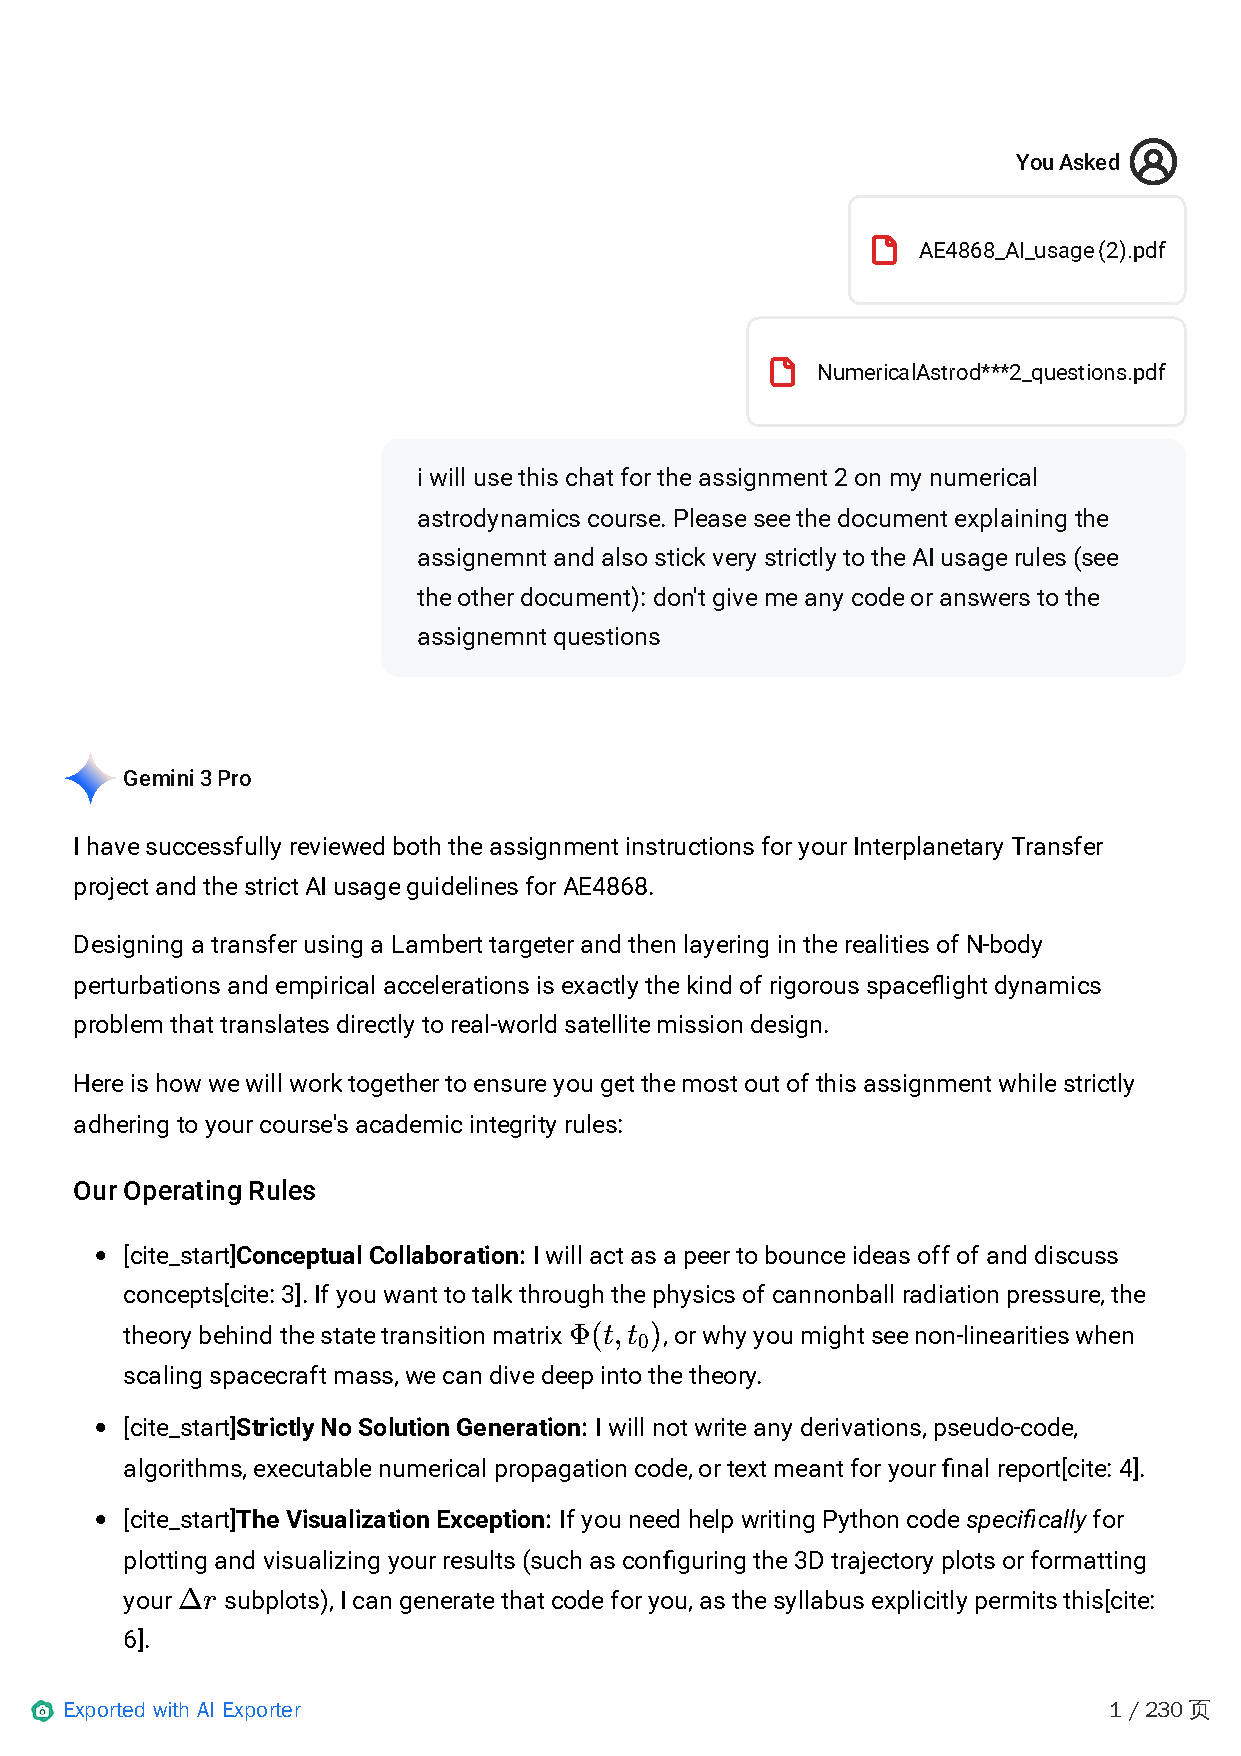
\includepdf[pages=-,pagecommand={},scale=0.95,frame=false]{Gemini-_22.pdf}

\end{document}